% !Mode:: "TeX:UTF-8"
% !TEX root = ../main.tex
\chapter{网格无关性分析和结果验证}\label{chap: validation}

\section{网格划分}\label{sec: grid}

\subsection{网格生成}

要计算的流动区域如图~\ref{fig: grid} 所示。将圆柱的直径设为 1;为了尽可能减少边界对流场的影响,将正方形的边长设为圆柱直径的 60 倍,并使圆柱位于正方形的中心位置。为了更好地生成网格,在圆内再划分出一个正方形,边长设为圆柱直径的一半。整个计算区域以圆为界,分为圆柱内部和圆柱外部两部分,内部为多孔介质区域,外部为纯流体区域,圆柱表面为多孔介质区和纯流体区的边界。
%由于采用结构化网格,每个网格均为四边形,为了使圆能被较好地划分,令圆内的网格更加规则,同时使圆柱表面内外的网格尽量光滑衔接,网格尺寸连续变化,

\begin{figure}
	\centering
	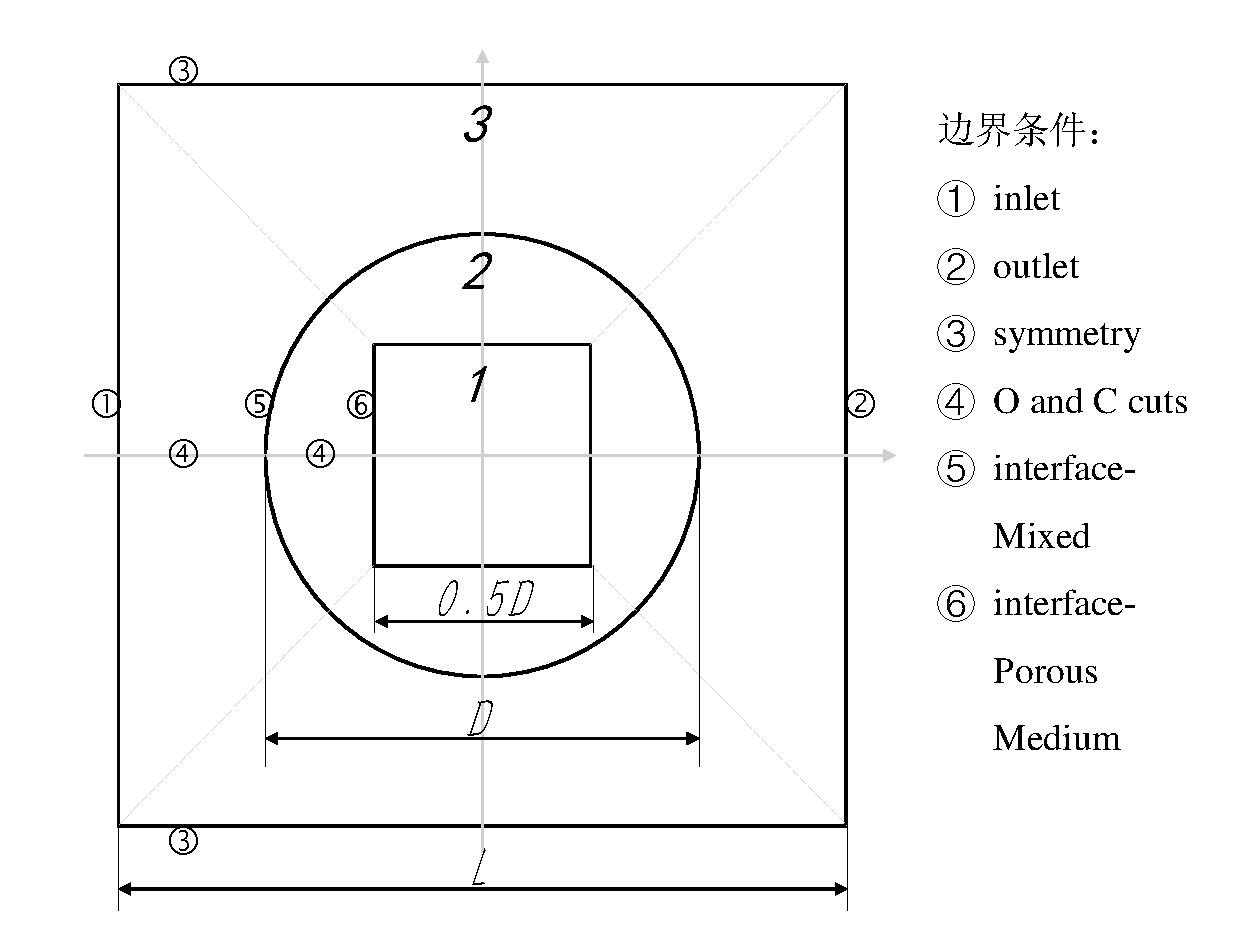
\includegraphics[scale=.7]{figs/grid}
	\caption{网格划分及边界条件设定}\label{fig: grid}
\end{figure}

在划分网格时,流动区域被分割为连续的小四边形,经纬两个方向的直线织成了整个平面区域。对于第一个子区域(圆内的正方形),只需要将四条边等分,再连接对应点即可。第二个子区域和第三个子区域为 O 型网格。第二个区域的内边界为正方形,外边界为圆,内外表面都被均匀划分,且取相同数量的节点,连接对应的节点形成一条条呈放射状的径向线段,将每一条线段等分,再顺次连接对应的节点,新得到的周向线段与之前的径向线段相交,形成了网状结构,区域被成功划分。第三个区域的内边界为圆,外边界为正方形,两个边界仍然是被均匀划分,连接节点形成径向直线,另一方向的网格划分也和第二个区域类似,不过径向线段不再被等分,而是按照内密外疏的原则依等比数列划分。为了保持圆内外两层网格的大小一致,第三个区域最内侧的网格密度比较大,如果均匀划分,将使网格数过多,而外部网格密度不需要太过细密,所以网格从内到外按照由密到疏的原则进行划分,等比数列是一个较好的选择。另外,为了使圆附近的网格更加细致,第二个区域可以按内疏外密将圆附近的网格适当加密,\ref{subsec: grid-independent}~小节第一组网格的第二个区域就是这样划分的。划分好的网格如图~\ref{fig: sketch of grid} 所示。

\begin{figure}
	\centering
	\subfigure[整个区域]{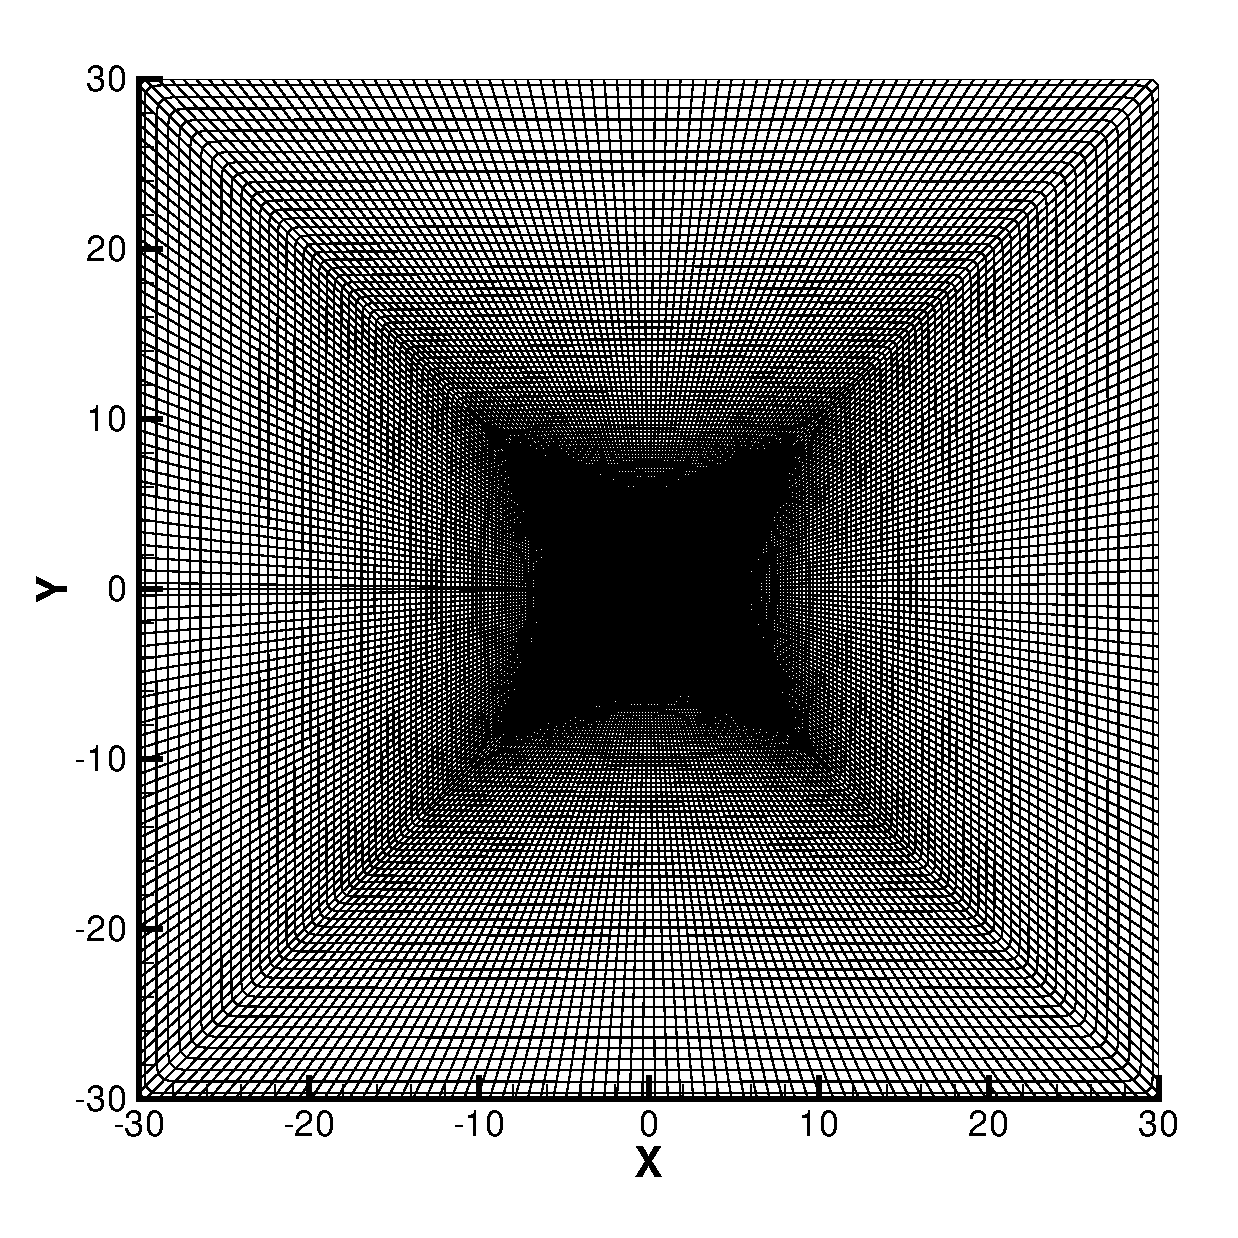
\includegraphics[width=0.47\textwidth]{figs/grid1}}
	\subfigure[圆柱附近]{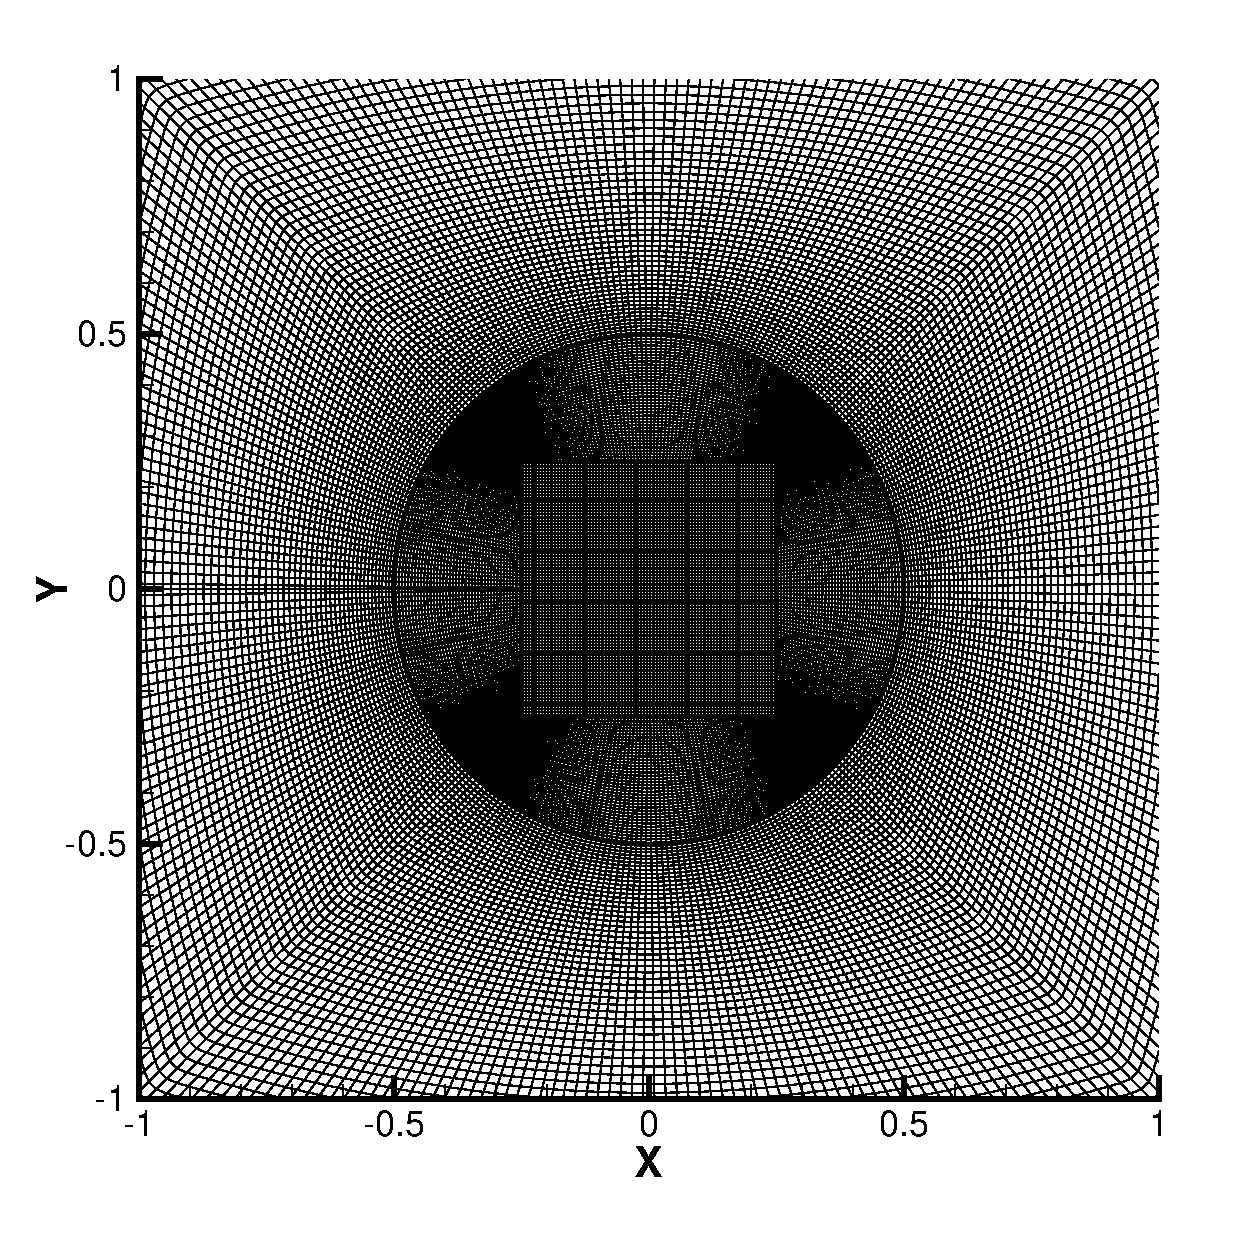
\includegraphics[width=0.47\textwidth]{figs/grid2}}
	\vspace{0.2em}
	\caption{实际计算网格示意图}\label{fig: sketch of grid}
\end{figure}

\subsection{网格无关性分析}\label{subsec: grid-independent}

解的精度依赖于网格的疏密程度,一般情况下,网格划分地越致密,解的精度也越高,但同时计算量也越大。最终应该取得平衡,在使解满足精度要求的同时,保持较高的计算效率,为此需要进行网格无关性验证。选择几种依次递增的网格密度,在同一条件、同一参数下进行数值计算,如果某一网格密度下的解与上一网格密度下的解之差满足精度要求,就认为解已足够精确,从而选择该网格密度作为数值模拟的设定值。计算采用的参数见表~\ref{tab: parameters},其中 $\Delta t$ 为计算过程中采用的时间步长。进行验证的雷诺数和达西数分别为 100 和 0.0001。计算结束后,根据数据得到的平均阻力系数见表~\ref{tab: grid}。表格的最后一列数值表示与上一行相比该行平均阻力系数的变化率。

同时设定四个样本点,搜集这四个位置各个物理量的信息,这四个点的坐标分别是 (0,0),(1,0),(3,0),(1.5,1.5)。通过记录样本点的速度、压强随时间的变化,便于后续分析。

从表~\ref{tab: grid} 可以看出,四种情形下计算得到的阻力系数已比较接近,但仍然存在一些差别,网格 2 的阻力系数比网格 1 增大了 0.58\%,网格 3 的阻力系数比网格 2 增大了 0.29\%,网格 4 的阻力系数比网格 3 减小了 0.36\%。因为网格 3 和 2 之间的差别已足够小,达到了 0.3\%,满足了精度要求,所以在后续计算中将采用网格 3 作为数值模拟过程中的网格密度。

\begin{table}[ht]
	\caption{计算参数的设定}\label{tab: parameters}
	\vspace{.5em}\centering\wuhao
	\begin{tabular}{*{8}{c}}
		\toprule[1.5pt]
		$D$ & $L$ & $U_{\infty}$ & $\rho$ & $\varepsilon$ & $\beta_1$ & $\beta_2$ & $\Delta t$\\
		\midrule[1pt]
		1 m & 60 m & 1 m/s & 1 $\mathrm{kg}/\mathrm{m}^3$ & 0.7 & 0 & 0 & 0.001 s\\
		\bottomrule[1.5pt]
	\end{tabular}
\end{table}

\begin{table}[ht]
	\caption{几种不同密度的网格尺寸及相应的阻力系数}\label{tab: grid}
	\vspace{.5em}\centering\wuhao
	\begin{tabular}{cccccc}
		\toprule[1.5pt]
		\multirow{2}[3]{*}{编号} & \multicolumn{3}{c}{网格尺寸} & \multirow{2}[3]{*}{平均阻力系数} & \multirow{2}[3]{*}{阻力系数变化率} \\
		\cmidrule[.67pt](lr){2-4}
		& 区域 1 & 区域 2 & 区域 3 & & \\
		\midrule[1pt]
		1 & 40 $\times$ 40 & 160 $\times$ 25 & 160 $\times$ 140 & 1.2354 & — \\
		2 & 60 $\times$ 60 & 240 $\times$ 30 & 240 $\times$ 170 & 1.2426 & 0.58\% \\
		3 & 80 $\times$ 80 & 320 $\times$ 40 & 320 $\times$ 200 & 1.2462 & 0.29\% \\
		4 & 100 $\times$ 100 & 400 $\times$ 50 & 400 $\times$ 230 & 1.2417 & $-0.36\%$ \\
		\bottomrule[1.5pt]
	\end{tabular}
\end{table}

\section{结果验证}\label{sec: result validation}

确定了网格密度之后,需要验证结果的准确性。已知在多孔圆柱绕流中,达西数决定了多孔介质中流动的程度,当达西数趋于无穷大时,多孔区域变成了纯流体区域,当达西数为零时,多孔区域则变成了固体区域,不再有流体的流动。所以,将达西数设成一个非常小的数值,如果得到的流动状态和已有文献中固体圆柱绕流的状态一致,说明结果是准确的。本文取 $Da=1\times 10^{-5}$ 进行验证。

通过计算得到了整个区域的流场特性,即速度、压力以及圆柱受到的阻力和升力等。根据某一物理量随时间变化的曲线可以得到无量纲频率 Strouhal 数。表~\ref{tab: validation} 列出了本文和过去文献中的一些计算结果,其中 $C_D$ 表示平均阻力系数,$C_{Dp}$ 表示压差引起的平均阻力系数,$C_{L'}$ 表示方均根升力系数。从表中可以看出,$Da=1\times 10^{-5}$ 时多孔圆柱中的流动已经接近于固体圆柱的情形,当前结果与已有结果基本一致。

%阻力系数和升力系数都随时间做周期性波动,对阻力系数取出一个周期内的平均值进行比较,升力系数的平均值为零,可以通过读取升力系数波动的振幅进行比较。在本文中,一些物理量采用以下约定符号表示。时间平均速度用平均符号($\bar{ }$)表示,例如 $\bar u$ 表示水平速度的时间平均值;方均根值通过撇号($^\prime$)来体现,例如 $u^\prime$ 表示水平速度的方均根值。平均阻力系数和平均升力系数分别用 $C_D$ 和 $C_L$ 表示(此处不再使用平均符号),并且都由压力和摩擦力共同引起:$C_D=C_{Dp}+C_{Df}$,$C_L=C_{Lp}+C_{Lf}$。阻力系数和升力系数的方均根值则分别表示为 $C_{D^\prime}$ 和 $C_{L^\prime}$。升力系数波动的振幅用 $C_L^A$ 表示。

\begin{table}[ht]
	\caption{和固体圆柱绕流数值结果的比较($Da=1\times 10^{-5}$,$Re=100$)}
	\label{tab: validation}
	\vspace{.5em}\centering\wuhao
	\begin{tabular}{*{5}{c}}
		\toprule[1.5pt]
		结果 & $St$ & $C_D$ & $C_{Dp}$ & $C_{L'}$ \\
		\midrule[1pt]
		Park et al. \inlinecite{Park1998} & 0.165 & 1.33 & 0.99 & 0.235 \\
		Li et al. \inlinecite{Li2009} & 0.164 & 1.336 & 0.995 & -- \\
		Harrichandan and Roy \inlinecite{Harichandan2010} & 0.161 & 1.352 & -- & -- \\
		Qu L \inlinecite{Qu2013} & 0.1648 & 1.319 & 0.984 & 0.225 \\
		Laroussi et al. \inlinecite{Laroussi2014} & 0.173 & 1.50 & -- & -- \\
		当前结果 & 0.1650 & 1.2724 & 0.9976 & 0.2232 \\
		\bottomrule[1.5pt]
	\end{tabular}
\end{table}

%Park 等人\cite{Park1998} 使用高分辨率的计算进行了模拟,

为了在整个雷诺数范围内作比较,展示出多孔介质趋于固体时的流动特性,将整个雷诺数范围内 Strouhal 数、平均阻力系数、升力系数振幅的变化和已有结果进行了比较,如图~\ref{fig: validation-St}、\ref{fig: validation-Cd} 和 \ref{fig: validation-Cl} 所示。

图~\ref{fig: validation-St} 显示了 Strouhal 数随雷诺数的变化,从图中可以看出,在雷诺数从 40 增大到 180 的范围内,当前结果与文献 \inlinecite{Williamson1996} 符合得比较好,$Re=180$ 和 $Re=200$ 两个点和文献不一致,可能是因为这时流动已具有三维特性,所以模拟的结果有一定偏差。

\begin{figure}
	\centering
	\includegraphics[width=0.8\textwidth]{../analysis/validation_St}
	\caption{Strouhal 数的对比}
	\label{fig: validation-St}
\end{figure}

图~\ref{fig: validation-Cd} 显示了平均阻力随雷诺数的变化,随着雷诺数的增大,平均阻力逐渐减小,且雷诺数在开始阶段减小很快,之后减小的速度慢慢变小,两条曲线都具有这一趋势,但与文献 \inlinecite{Rajani2009} 有一定的差距,而且文献中的数据在 $Re=60$ 之前下降很快,随后却由一个明显的上升,然后才缓慢下降,这导致曲线在 $Re=60$ 附近不连续,原因尚不明确,可能这是由两段数据组合而成的一个直线。此外,当前研究和文献数据在阻力值上的差距也不明确,只是总体上具有相同的变化趋势。如果在程序中不考虑达西数,而不是将达西数设为一个很小的值,那么得到的结果会更接近文献数据。所以,这一差距可能由达西数的加入而引起。

\begin{figure}[ht]
	\centering
	\includegraphics[width=0.8\textwidth]{../analysis/validation_Cd}
	\caption{平均阻力系数 $C_D$ 的对比}
	\label{fig: validation-Cd}
\end{figure}

图~\ref{fig: validation-Cl} 显示了升力振幅随雷诺数的变化,升力波动的振幅均随雷诺数的增大而增大,且二者基本吻合。总体而言,当前结果与文献在一定程度上是一致的,经过验证,结果基本准确。

\begin{figure}[t]
	\centering
	\includegraphics[width=0.8\textwidth]{../analysis/validation_Cl}
	\caption{升力系数 $C_L$ 的对比}
	\label{fig: validation-Cl}
\end{figure}

\section{本章小结}

本章对个别多孔圆柱绕流情形进行了计算,确定了网格的划分形式以及计算所需的网格分辨率,和固体绕流的结果进行对比,验证了计算结果的准确性。

\ref{sec: grid} 节定义了该问题的计算区域,将正方形的计算区域划分为三个子域,在每个区域内划分出正交网格,并规定每两块网格之间的边界条件。为了寻找合适的网格分辨率,在取得足够精度的同时又保证一定计算效率,进行了网格无关性验证。固定其他参数,设定一系列的网格密度,分别计算,对得到的结果进行分析,发现 $80\times 80$ 的网格具有足够的精度,将作为后续计算的设定。

\ref{sec: result validation} 节计算了 $Da=1\times 10^{-5}$、$Re=100$ 时的流动情形,将得到的各物理量的变化情况和已有的固体圆柱绕流结果比对,确定了计算的准确性。
